\todo[inline]{Add top padding for scenario tables} 
\section{Use case scenarios}
Now we are going to depict goals of users which the application will make achievable.
Figure 2.1 contains a use case diagram of the application.
A use case styled with a bold border groups together more use cases and will be further expanded.
All use cases will be structurally described by independent use case scenarios.
A scenario will contain its description only if the goal of a user is not clear from a use case's name.

\begin{figure}[h]
  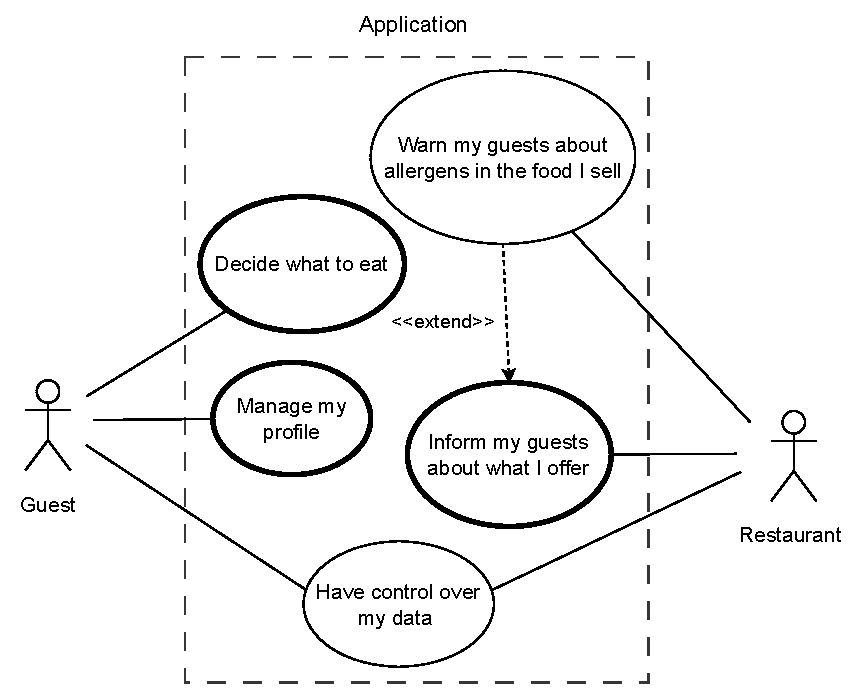
\includegraphics[width=\linewidth]{master-thesis/img/use-cases/use_cases}
  \caption{The application's use case diagram.}
\end{figure}

\newpage

\def\arraystretch{1.5}

\subsection{Guest use cases}
\todo[inline]{change name in figure}
\textbf{UC1: Decide what to order}
\begin{center}
  \begin{tabular}{| l | p{10.75cm} | }
    \hline
    Actor        & Guest \\
    \hline
    Description  & A guest comes to a restaurant and is deciding what to order. \\
    \hline
    Covers & R1.5-R1.9, R1.16 \\
    \hline
    Precondition & The guest has opened a restaurant's menu using the application. \\
    \hline
    Postcondition & The guest is viewing a personalized menu. \\
    \hline
    Scenario     &
    \begin{minipage}[t]{\linewidth}
      \begin{enumerate}[leftmargin=*,nosep,before=\vspace{-0.575\baselineskip},after=\strut]
        \item The guest logs in to the application. \textbf{A1}
        \item The application loads the guest's profile.
        \item The application applies the guest's preferences to the menu.
        \item The application displays the menu enriched with visual clues so that the guest can see what they can and cannot eat.
        \item The guest selects to divide the menu to items they can and items they cannot eat. \textbf{A2 A3}
        \item The application restructures the menu.
      \end{enumerate}
    \end{minipage}
    \\
    \hline
    Alternatives &
    \begin{minipage}[t]{\linewidth}
      \begin{description}[nosep,after=\strut]
        \item [A1:] The guest does not log in. The guest selects what they are allergic to and what diets they follow using controls in the menu. The scenario continues with step 3.
        \item [A2:] The guest selects to sort the menu by whether they can eat an item.
        \item [A3:] The guest selects to filter out items which they cannot eat.
      \end{description}
    \end{minipage}
    \\
    \hline
  \end{tabular}
  \newline
\end{center}

\begin{figure}[h]
  \centering
  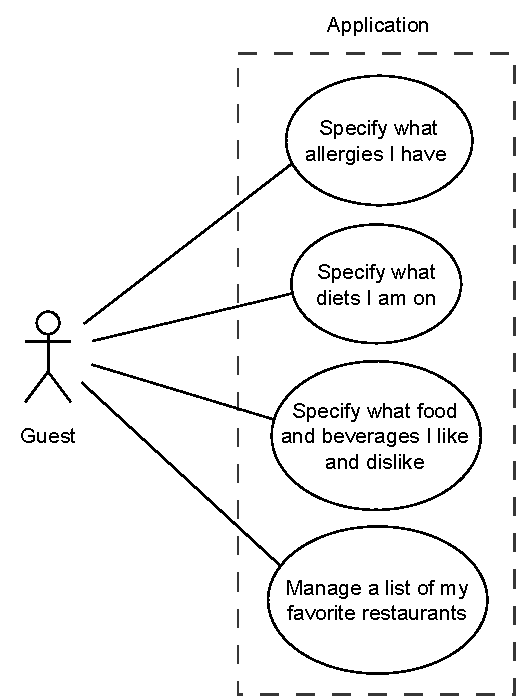
\includegraphics[width=0.62\linewidth]{master-thesis/img/use-cases/use_cases_guest_profile_management}
  \caption{Guest profile management use cases}
\end{figure}

\newpage

\todo[inline]{change name in figure}
\noindent \textbf{UC2: Specify what I am allergic to}
\begin{center}
  \begin{tabular}{| l | p{10.75cm} | }
    \hline
    Actor         & Guest \\
    \hline
    Covers        & R1.1, R1.4 \\
    \hline
    Precondition  & The guest is logged in to the application. \\
    \hline
    Postcondition & The guest's profile contains data about what the guest is allergic to. \\
    \hline
    Scenario      &
    \begin{minipage}[t]{\linewidth}
      \begin{enumerate}[leftmargin=*,nosep,before=\vspace{-0.575\baselineskip},after=\strut]
        \item The guest opens their profile.
        \item The application displays options for what a person can be allergic to.
        \item The guest selects options based on what they are allergic to. \textbf{A1}
        \item The guest presses a button for saving their profile.
        \item The application updates the guest's profile.
      \end{enumerate}
    \end{minipage}
    \\
    \hline
    Alternatives &
    \begin{minipage}[t]{\linewidth}
      \begin{description}[nosep,after=\strut]
        \item [A1:] Some of the options are selected because the guest has already specified them in the past.
      \end{description}
    \end{minipage}
    \\
    \hline
  \end{tabular}
  \newline
\end{center}

\noindent \textbf{UC3: Look up online what a restaurant offers today}
\begin{center}
  \begin{tabular}{| l | p{10.75cm} | }
    \hline
    Actor        & Guest \\
    \hline
    Description  & A guest wants to know what a restaurant serves at the moment. \\
    \hline
    Covers        & R1.10-R1.12, R1.15, R1.16 \\
    \hline
    Precondition  & The guest has access to the internet. \\
    \hline
    Postcondition & The guest sees a current menu of the restaurant. \\
    \hline
    Scenario     &
    \begin{minipage}[t]{\linewidth}
      \begin{enumerate}[leftmargin=*,nosep,before=\vspace{-0.575\baselineskip},after=\strut]
        \item The guest searches for the restaurant by its name. \textbf{A1 A2 A3 A4}
        \item The application displays the restaurant's detail which contains a list of its menus.
        \item The guest selects a menu.
        \item The application displays the menu. \textbf{A5}         
      \end{enumerate}
    \end{minipage}
    \\
    \hline
    Alternatives &
    \begin{minipage}[t]{\linewidth}
      \begin{description}[nosep,after=\strut] 
        \item [A1:] The guest selects the restaurant in the overview screen from UC4.
        \item [A2:] The guest visits the restaurant's webpage and clicks on a link which takes them to the application.
        \item [A3:] The guest scans a QR code on a printed menu which takes them to the application.
        \item [A4:] The guest specifies the IRI of the restaurant. 
        \item [A5:] The application first translates the menu into the current language of the user interface. 
      \end{description}
    \end{minipage}
    \\
    \hline
  \end{tabular}
  \newline
\end{center}

\newpage

\begin{figure}[h]
  \centering
  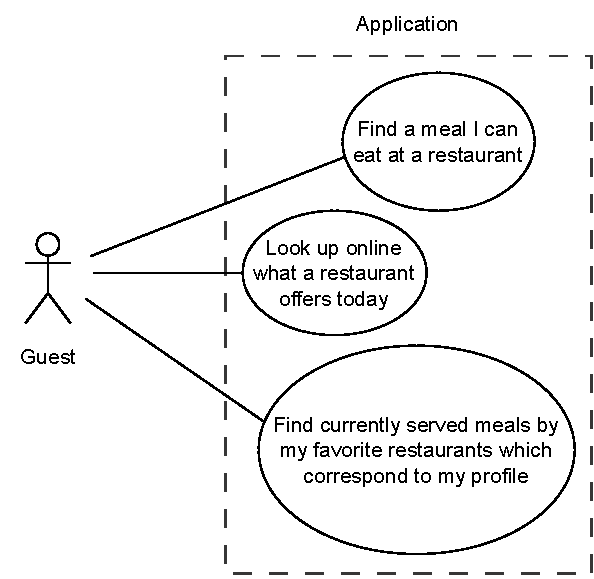
\includegraphics[width=0.62\linewidth]{master-thesis/img/use-cases/use_cases_guest_menu_viewer}
  \caption{Guest menu viewing use cases}
\end{figure}

\todo[inline]{change name in figure}
\noindent \textbf{UC4: See currently served meals by my favorite restaurants which I can eat}
\begin{center}
  \begin{tabular}{| l | p{10.75cm} | }
    \hline
    Actor        & Guest \\
    \hline
    Description  & A guest wants to know what do their favorite restaurants currently offer. \\
    \hline
    Covers & R1.14 \\
    \hline
    Precondition & The guest is logged in to the application. \\
    \hline
    Postcondition & The guest sees an overview of what the guest's favorite restaurants currently serve. \\
    \hline
    Scenario     &
    \begin{minipage}[t]{\linewidth}
      \begin{enumerate}[leftmargin=*,nosep,before=\vspace{-0.575\baselineskip},after=\strut]
        \item The application displays a list of the guest's favorite restaurants with selected items from their menus. \textbf{A1}\textbf{A2} \textbf{A3}
      \end{enumerate}
    \end{minipage}
    \\
    \hline
    Alternatives &
    \begin{minipage}[t]{\linewidth}
      \begin{description}[nosep,after=\strut]
        \item [A1:] The overview is empty because the restaurants do not currently serve anything. The application displays a text with this information.
        \item [A2:] The overview is empty because the guest has not added any favorite restaurants yet. The application displays instructions on how to add a restaurant to the list.
        \item [A2:] One of the favorite restaurants has no valid menu published at the moment. The application displays a text with this information close to the restaurant's name.
      \end{description}
    \end{minipage}
    \\
    \hline
  \end{tabular}
  \newline
\end{center}

\newpage

\noindent \textbf{UC5: Specify what diets I am on}
\begin{center}
  \begin{tabular}{| l | p{10.75cm} | }
    \hline
    Actor       & Guest \\
    \hline
    Covers & R1.2, R1.4 \\
    \hline
    Precondition  & The guest is logged in to the application. \\
    \hline
    Postcondition & The guest's profile contains data about what diets is the guest on. \\
    \hline
    Scenario    &
    \begin{minipage}[t]{\linewidth}
      \begin{enumerate}[leftmargin=*,nosep,before=\vspace{-0.575\baselineskip},after=\strut]
        \item The guest opens their profile.
        \item The application displays a screen with a list of previously specified diets by the guest. \textbf{A1}
        \item The guest presses a button for adding a new diet to the list.
        \item The application displays a search bar.
        \item The guest starts typing the name of a diet into the search bar.
        \item The application suggests diets which contain the given input in their name.
        \item The guest selects the desired diet. \textbf{A2}
        \item The application adds the diet to the guest's profile. \textbf{A3}
        \item The guest repeats steps 3 to 8 until they have specified all of the diets they are on.
      \end{enumerate}
    \end{minipage}
    \\
    \hline
    Alternatives &
    \begin{minipage}[t]{\linewidth}
      \begin{description}[nosep,after=\strut]
        \item [A1:] The list is empty because the guest has not specified any diets yet. The application displays a text containing this information.
        \item [A2:] The application does not recognize the diet which the guest is trying to specify. The guest creates a public issue in the application's repository with a request to add the desired diet to the application.
        \item [A3:] The diet the guest has specified is already contained in the guest's profile. The application informs the guest about this fact and their profile is not altered.
      \end{description}
    \end{minipage}
    \\
    \hline
  \end{tabular}
  \newline
\end{center}

\todo[inline]{add covering of nonfunctional req.}
\noindent \textbf{UC6: Have control over my data}
\begin{center}
  \begin{tabular}{| l | p{10.75cm} | }
    \hline
    Actor        & Guest \\
    \hline
    Description  & A guest wants to specify where should the application store their data. \\
    \hline
    Covers & R3.7 \\
    \hline
    Precondition  & The guest is logged in to the application. \\
    \hline
    Postcondition & The application uses the storage space chosen by the guest for storing and accessing the guest's data. \\
    \hline
    Scenario     &
    \begin{minipage}[t]{\linewidth}
      \begin{enumerate}[leftmargin=*,nosep,before=\vspace{-0.575\baselineskip},after=\strut]
        \item The guest navigates to a page for managing data storage options.
        \item The application provides a list of options where it can store the guest's data. \textbf{A1}
        \item The guest selects one of the options.
        \item The application starts using the selected place for storing and reading the guest's data.
      \end{enumerate}
    \end{minipage}
    \\
    \hline
    Alternatives &
    \begin{minipage}[t]{\linewidth}
      \begin{description}[nosep,after=\strut]
        \item [A1:] There is only one option in the list. The guest cannot change the option.
      \end{description}
    \end{minipage}
    \\
    \hline
  \end{tabular}
  \newline
\end{center}

\newpage

\todo[inline]{Decide whether to use "A guest" or "The guest" in all descriptions}
\todo[inline]{Change "the application displays a screen with a list" to "the application displays a list" in other reqs}
\todo[inline]{Update name in figure}
\todo[inline]{Change scenario so that the applicaton saves the profile after all of the foods and ingredients are specified - not after every food specified - also in UC about specifying diets}
\todo[inline]{there is a search bar next to the list of foods which the guest likes. The guest starts typing into the searchbar, chooses a food and clicks a button for adding it to the list}
\todo[inline]{the guest does not create a public issue (this is subject of design) - the application provides information about how to request adding a food or ingredient to the application}
\noindent \textbf{UC7: Specify what foods I like and dislike}
\begin{center}
  \begin{tabular}{| l | p{10.75cm} | }
    \hline
    Actor    & Guest \\
    \hline
    Description & A guest wants to specify their taste preferences so that they are taken into account when the guest is viewing a restaurant's menu. \\
    \hline
    Covers & R1.3, R1.4 \\
    \hline
    Precondition  & The guest is logged in to the application. \\
    \hline
    Postcondition & The guest's profile contains data about what foods and ingredients the guest likes and dislikes. \\
    \hline
    Scenario &
    \begin{minipage}[t]{\linewidth}
      \begin{enumerate}[leftmargin=*,nosep,before=\vspace{-0.575\baselineskip},after=\strut]
        \item The guest opens their profile.
        \item The application displays two lists, one containing the foods and ingredients which the guest likes and the other containing the foods and ingredients which the guest dislikes. \textbf{A1}
        \item The guest presses a button for adding an item to the list of the foods and ingredients which they like. \textbf{A2}
        \item The application displays a search bar.
        \item The guest starts typing the name of a food or ingredient into the search bar.
        \item The application suggests foods and ingredients which contain the given text in their name.
        \item The guest selects the desired food or ingredient and presses a button for adding it to the list. \textbf{A3}
        \item The applicaton updates the list.
        \item The guest repeats steps 3 to 8 until they have specified all of their food preferences.
        \item The guest presses a button for saving their profile.
        \item The application saves the guest's profile. 
      \end{enumerate}
    \end{minipage}
    \\
    \hline
    Alternatives &
    \begin{minipage}[t]{\linewidth}
      \begin{description}[nosep,after=\strut]
        \item [A1:] Either one or both of the lists are empty because the guest has not specified any of their preferences yet. The application displays a text which informs the guest about this fact.
        \item [A2:] The guest presses a button for adding an item to the list of the foods and ingredients which they dislike.
        \item [A3:] The application does not recognize the food which the guest is trying to specify. The guest creates a public issue in the application's repository with a request to add the desired food to the application.
      \end{description}
    \end{minipage}
    \\
    \hline
  \end{tabular}
  \newline
\end{center}

\newpage

\todo[inline]{check in other use cases whether I used ',' between A1 and A2}
\todo[inline]{search field is already next to the list, the guest types the name and clicks "Add" to the list}
\noindent \textbf{UC8: Manage a list of my favorite restaurants}
\begin{center}
  \begin{tabular}{| l | p{10.75cm} | }
    \hline
    Actor    & Guest \\
    \hline
    Covers & R1.13 \\
    \hline
    Precondition & The guest is logged in to the application. \\
    \hline
    Postcondition & A restaurant is added to the list of the guest's favorite restaurants. \\
    \hline
    Scenario &
    \begin{minipage}[t]{\linewidth}
      \begin{enumerate}[leftmargin=*,nosep,before=\vspace{-0.575\baselineskip},after=\strut]
        \item The application displays a list of the guest's favorite restaurants. \textbf{A1 A2}  
        \item The guest presses the button for adding a restaurant to the list. \textbf{A3}
        \item The application displays a text input field.
        \item The guest starts typing the name of the restaurant. \textbf{A4}  
        \item The application suggests restaurants which contain the specified text in their name to the user. 
        \item The guest clicks on a restaurant's name. \textbf{A5}
        \item The application adds the selected restaurant to the list.
        \item The guest repeats steps 2 to 7 until they are satisfied with the content of the list.
        \item The guest presses a button for saving their profile.
        \item The application saves the guest's profile.
      \end{enumerate}
    \end{minipage}
    \\
    \hline
    Alternatives &
    \begin{minipage}[t]{\linewidth}
      \begin{description}[nosep,after=\strut]
        \item [A1:] The guest is viewing a restaurant's detail. The guest presses the button for marking the restaurant as their favorite. The application adds the restaurant to the guest's profile. \textbf{A1.b}
        \item [A1.b:] The restaurant is already contained in the guest's profile and pressing the button removes the restaurant from it.
        \item [A2:] The list is empty because the guest has not added any restaurants yet. The application displays a text with this information.
        \item [A3:] The guest presses a button for removing a restaurant. The application removes the restaurant from the list.
        \item [A4:] The guest specifies the restaurant's IRI. \textbf{A3.b}   
        \item [A4.b:] The IRI which the guest specified is not valid. The application informs the guest about this fact and the scenario continues with step 4.
        \item [A5:] The application did not find the desired restaurant because it does not use our application. The application displays a text saying that it was not able to find any restaurants by the specified name. The scenario ends.
      \end{description}
    \end{minipage}
    \\
    \hline
  \end{tabular}
  \newline
\end{center}

\newpage